\chapter{Design Choices}
\label{chapter:design}

\section{Introduction}
\label{section:introduction}
For a start, the design of the learning environment will be investigated more closely. First, the two possibilities for the main implementation structure will be presented. Then, the decisions of less general implementation techniques will be pointed out, and lastly, some graphical design details will be taken into consideration.

\section{Design Research}
\label{section:designchoice}
Before the project was launched, some research had to be done such as the acquisition of knowledge and implementation techniques in order to avoid common mistakes. Planning is a fundamental step in building a successful learning environment. The most general choices that have to be made in the beginning can support the creation of different exercises or features or heavily handicap this process. The research that had to be done included the following topics, listed in descending order, starting from the most fundamental and general choice: 

\begin{itemize}
\item Choice of the web framework
\item Choice of the underlying programming language
\item Choice of the graphical user interface (GUI)
\item Choice of the technical structure of the learning environment
\item Choice of the practical structure of the learning environment
\item Choice of the graphical design
\end{itemize}
In the following, the design choices based on research results will be presented. This will help to understand the general structure of the project and lays the foundation to understand the learning environment architecture in the following chapter.

\section{Choice of the Web Framework}
\label{section:designchoice}
In the beginning of the project, major decisions on how to design and implement the learning environment were to be taken. At ABZ, there were already several learning environments in use when this project was about to start. One major requirement of the newly created environment was that it can be embedded or connected with an already existing environment. As a first step, research on these already existing platforms had to be done. This included meetings with programmers and maintenance personnel, as well as technical research on implementation options and techniques was carried out. 

Other learning environments from ETH \cite{L1} and private organizations were analysed as inspiration for the design and functionality. For example, the online platform called Hamsterkiste \cite{L2} and an even bigger environment with name Schlaukopf \cite{L3} were taken into consideration. Soon, two options emerged that could be considered realistic and reasonable. The two options will be examined more closely in the following sections.

\subsection{Option 1}
One possibility to move on was to embed the newly created platform into the already existing programming environment from ABZ \cite{SBT}. Within this given framework, new tasks can be created and added. The functionality and design choices of this framework are, however, restrictive. The design of the task is fixed and the scope of new functions is heavily limited  (see examples in figures \ref{fig:P11} and  \ref{fig:P12}). 


\begin{figure}[H]
    \centering
    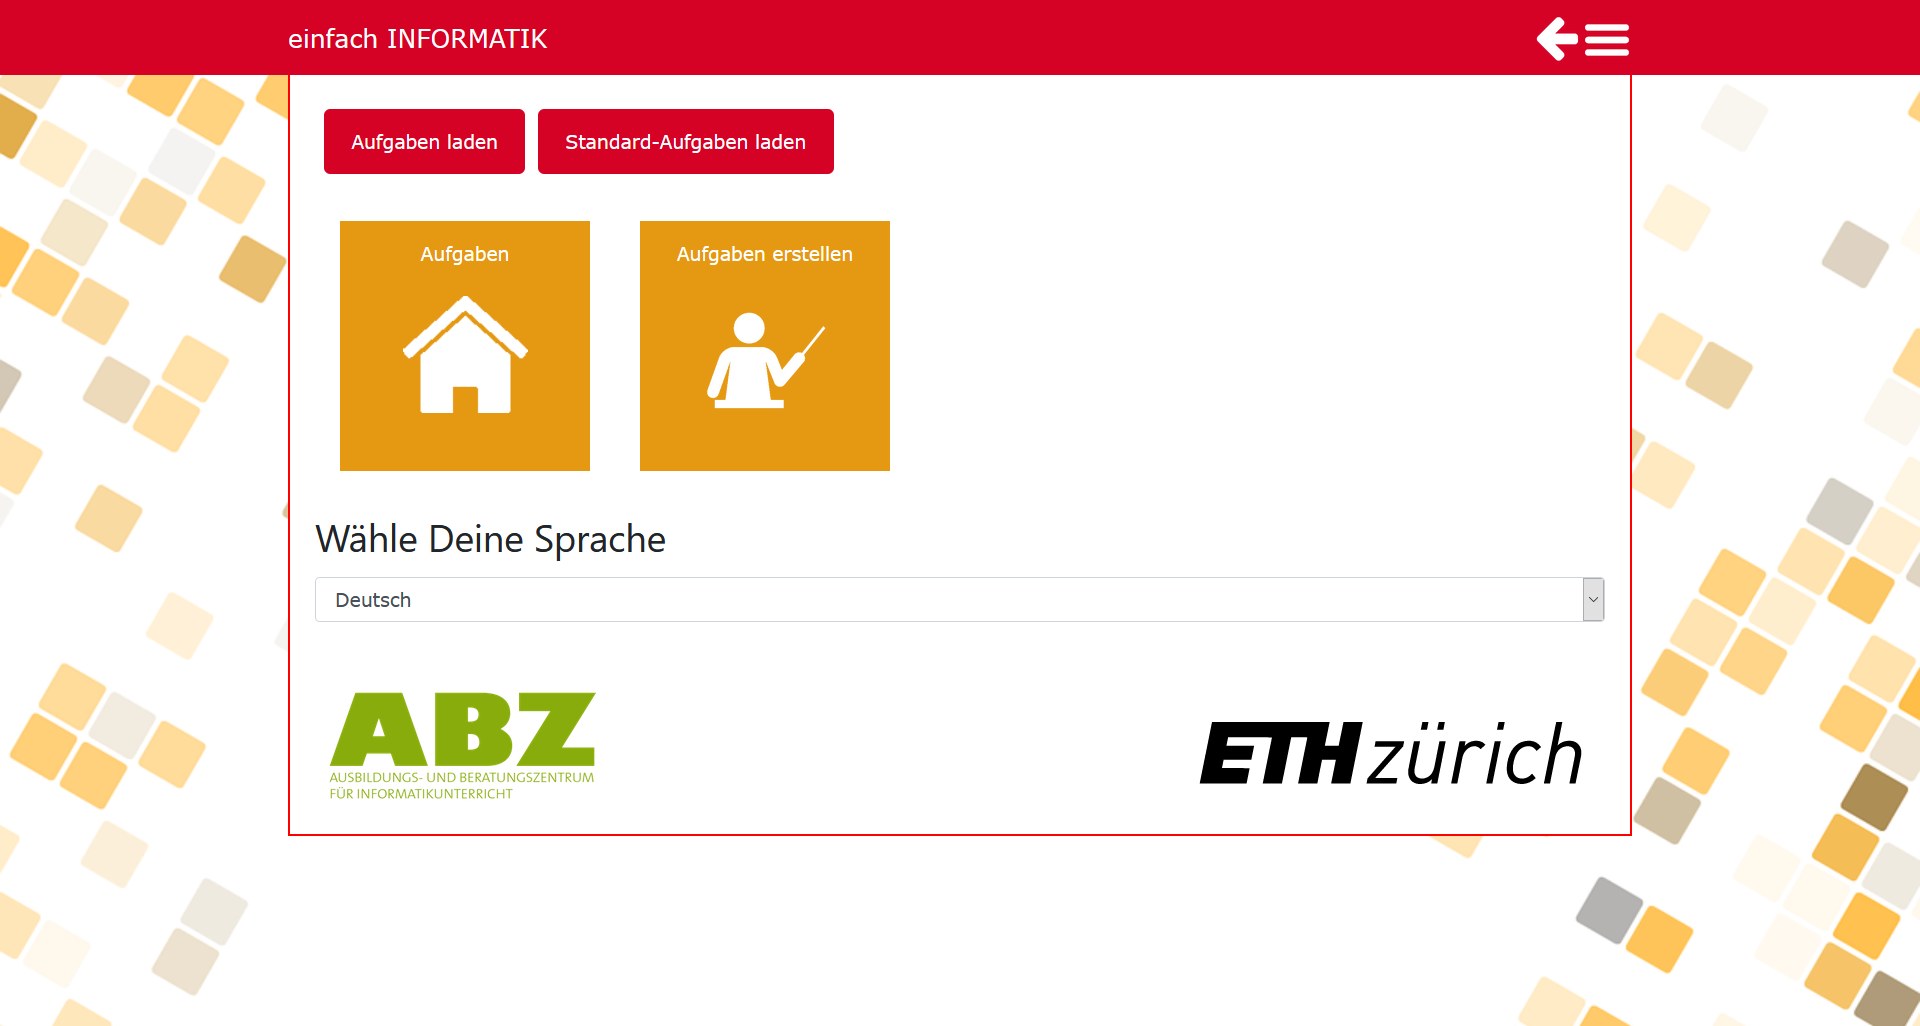
\includegraphics[width=1.0\columnwidth]{figures/P12.png}
    \caption{Home Page of Option 1}
    \label{fig:P11} 
\end{figure}

\begin{figure}[H]
    \centering
    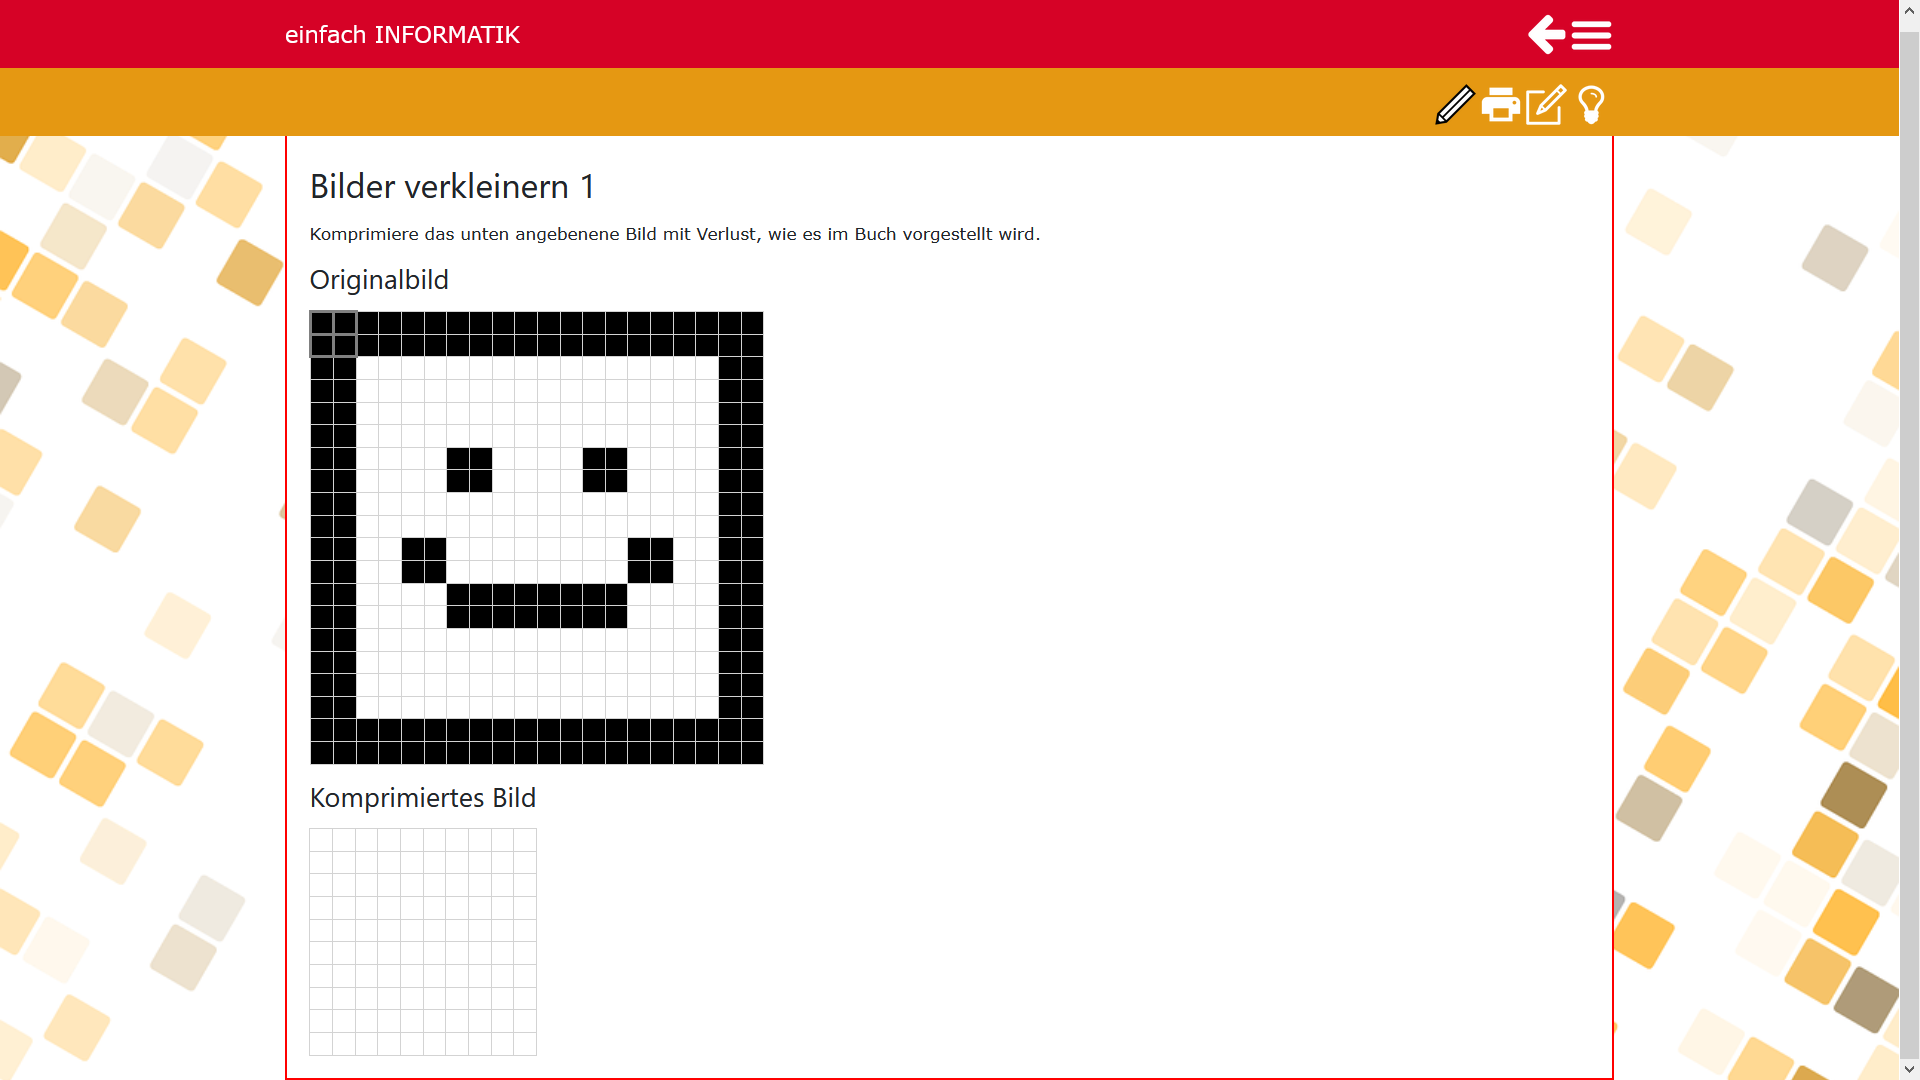
\includegraphics[width=1.0\columnwidth]{figures/P11.png}
    \caption{In-Game Snapshot of Option 1}
    \label{fig:P12} 
\end{figure}

\newpage
\subsection{Option 2}
The alternative to embedding the project into ABZ's framework was to create a new environment from scratch that then can easily be connected with the other environments for "einfach Informatik 3/4" that are about to emerge. The advantage of this choice is that a new project for the age group of third and fourth grade has been successfully completed and launched \cite{FBBT}. This project is more user-friendly and better adapted to the age group (see figures \ref{fig:P21} and  \ref{fig:P22}).

\begin{figure}[H]
    \centering
    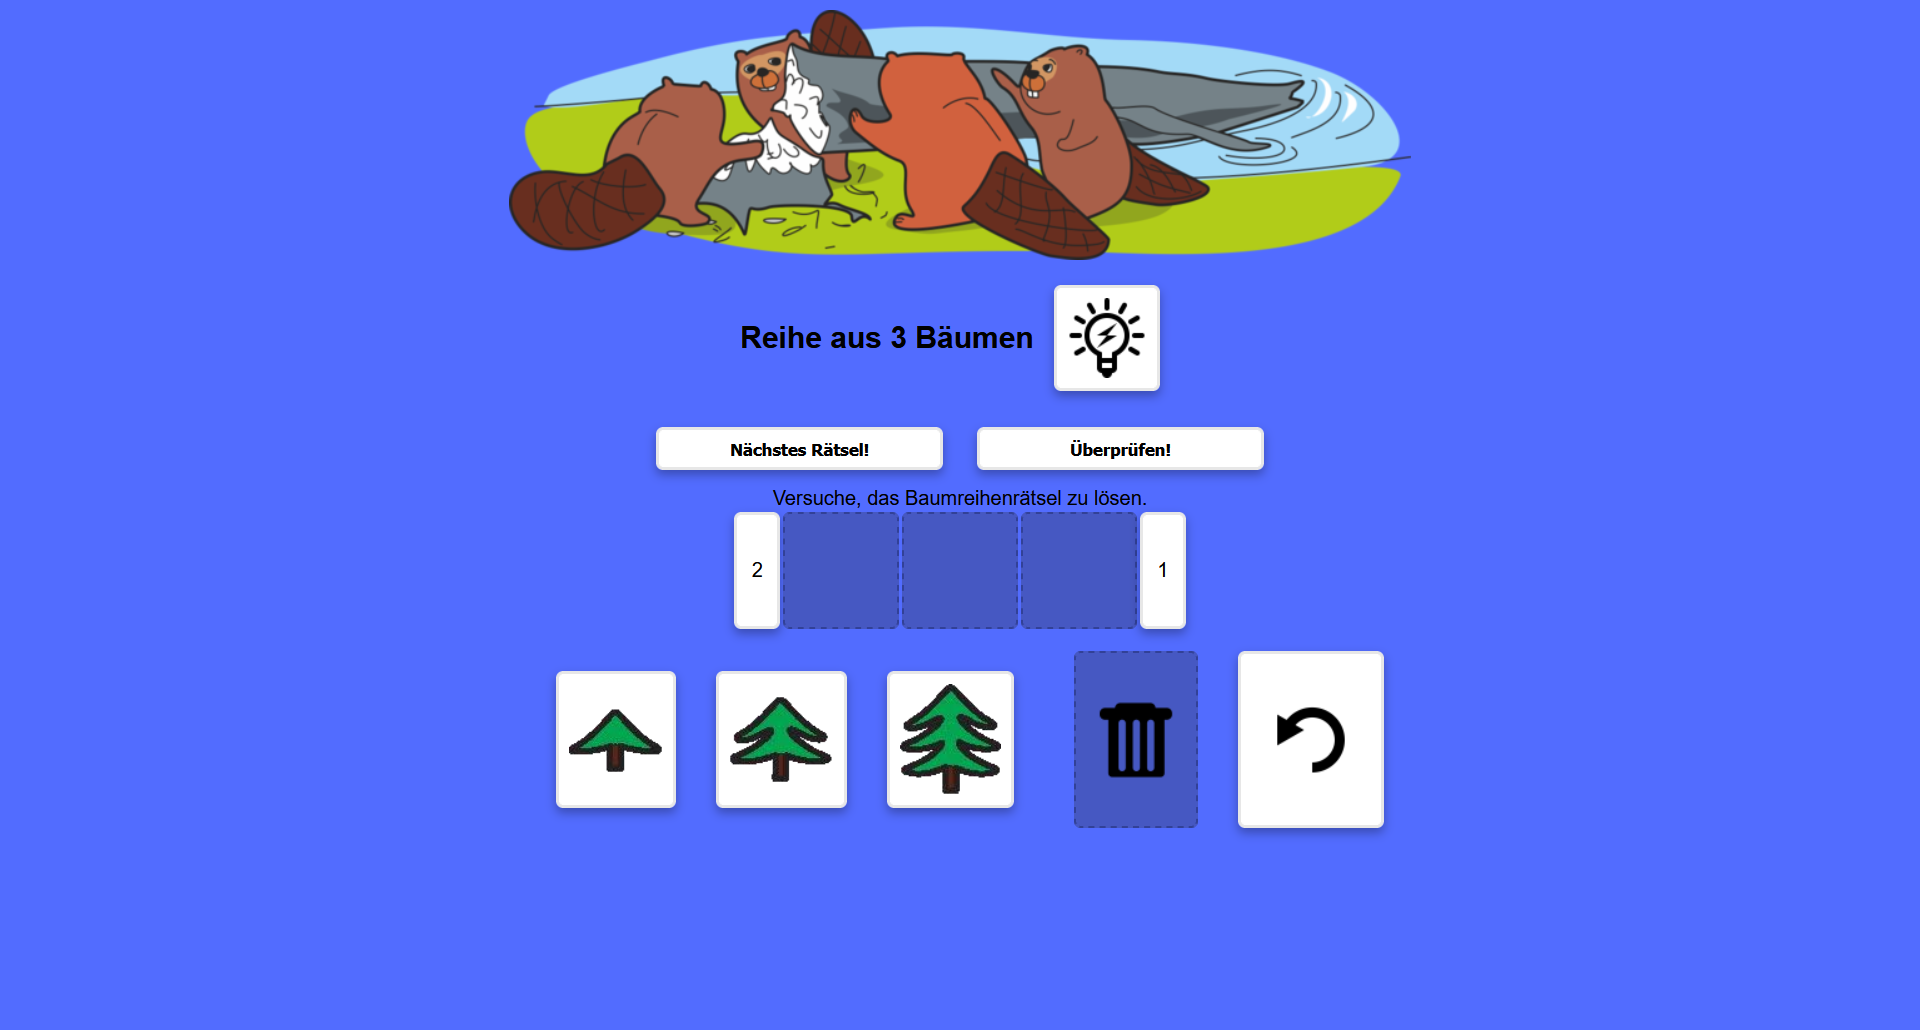
\includegraphics[width=1.0\columnwidth]{figures/P21.png}
    \caption{Home Page of Option 2}
    \label{fig:P21} 
\end{figure}

\begin{figure}[H]
    \centering
    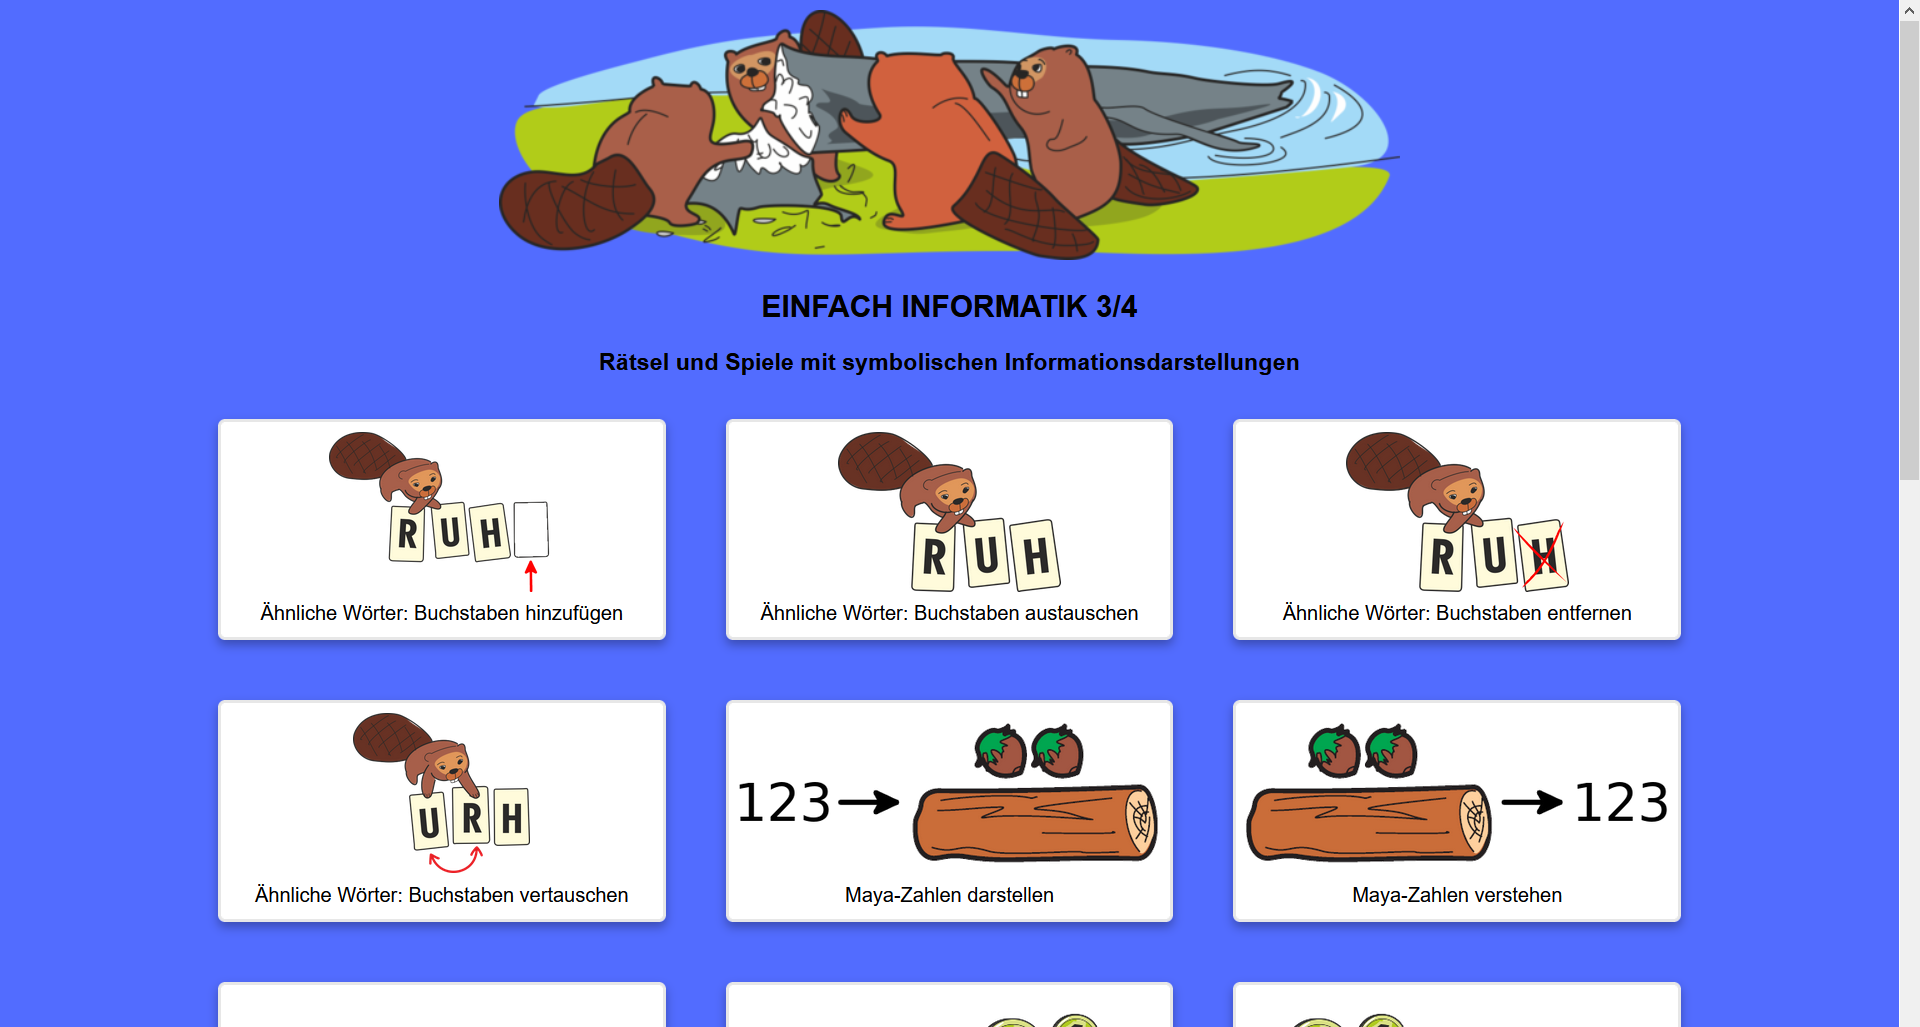
\includegraphics[width=1.0\columnwidth]{figures/P22.png}
    \caption{In-Game Snapshot of Option 2}
    \label{fig:P22} 
\end{figure}

\subsection{Decision and Justification}
The choice was made to build up a new environment according to option 2 in order to keep the freedom to program games without restrictions and to create a design that is appealing for third and fourth graders. Thereby, the interconnection to the already existing environment for "einfach Informatik 3/4" \cite{FBBT} is facilitated by this choice.

\section{Vue.js}
\label{section:vuejs}
The obvious choice to implement option 2 was to choose Vue.js as the main framework. Vue.js is a web framework developed several years ago by Evan You. It is built on top of JavaScript and features reactivity, which means that changes to the data of the application are directly applied and can immediately be seen by the user. Also, Vue.js features direct bi-directional communication between two components, given that they are in direct relation \cite{Vue}. The aforementioned features are major advantages when designing game-like tasks, as in this project. The main reason for this web framework was its simplicity in comparison to alternatives like Angular or React, and the fact that the existing environment for "einfach Informatik 3/4" also runs on Vue.js \cite{FBBT}.

Since the newest Vue.js version 3.0 was only a few months old when the project was launched, the choice was made to stick to the older version, namely version 2. This way, it was possible to ensure full library and web forum support. Version 2 has been established and proven itself as a solid framework for web applications \cite{Vue}.


\section{TypeScript}
\label{section:typescript}

For the choice of the underlying programming language, there were two options that are compatible with Vue.js: JavaScript and TypeScript. TypeScript was chosen since it is an extension to JavaScript and provides some additional functions. 

The latter is a scripting language that is dynamically typed. Informally, JavaScript helps to control how the website behaves. It can be used in browsers and runs on top of HTML and CSS, which are manipulated to enhance the user experience. JavaScript can receive, manipulate, and send data. JavaScript does not run on the server where all the information of a website is stored but on the user's computer, so it is run on client-side programming language. This leads to a shift of the workload and computational resources \cite{Javascript}. 

TypeScript extends JavaScript by providing type safety and concepts such as interfaces, method signatures, interfaces, enumerations and tuples. It provides a way to describe what type a variable has and helps to catch errors before the code is run. The type safety is assured during compilation from TypeScript to JavaScript \cite{Typescript}.

\section{HTML and CSS}
\label{subsection:html}
The choice of how to model the graphical interface was made along with the two previous choices. The common technologies for web development are HTML5 and CSS. HTML and CSS are core technologies that help building a website. They allow the developer to display program elements visually such that it can be seen by an end user. HTML is a descriptive language that enables the programmer to structure a website. CSS allows the software engineer to design and style a page in terms of colours, layouts, and fonts. JavaScript animates the content created by HTML and CSS files.

\section{Code Conventions}
As mentioned before, the design choices should support compatibility with other learning environments. Therefore, the technical structure of the learning environment is of fundamental importance.
The way code was written was adapted to some common, yet unofficial rules. The following list is a shortened citation of the documentation of the already existing learning framework for 'einfach Informatik 3/4' \cite{FBWT}. It represents some code conventions that help keeping a clean code structure and provide better readability. For each convention, code examples can be found in the Vue.js style guide \cite{VueStyleGuide}.

\begin{itemize}
    \item Always use \code{key} with \code{v-for} to maintain the internal component state.
    \item Avoid \code{v-if} with \code{v-for}
    \item Only the top-level \code{App} component and layout components should have global styles. All other components should always have scoped styles i.e. the style is only used within the component.
    \item Each component has its own file.
    \item Filenames are in PascalCase.
    \item Components without any content should be self-closing e.g \code{<Component />} instead of \code{<Component><Component/>}.
    \item Components name casing in templates is PascalCase.
    \item Properties name casing is camelCase.
    \item Elements with multiple attributes should span multiple lines, with one attribute on each line. [...]
    \item Element attribute values should be quoted.
    \item Directive shorthands are always used.
    \item Element attributes should be ordered consistently.
    \item Components should be ordered like \code{<templates>}, \code{<script>} and \code{<style>}.
    \item Element selectors should be avoided with \code{scoped}
    \item Properties and events should be used for parent-child communication.\cite{FBWT}
\end{itemize}

\section{Graphical Design}
The graphical design was chosen according to several criteria.
The fundamental criterion was that the design of the environment is intuitive and child-friendly. The young students should understand the functionality of the platform as good as possible. To facilitate this, the design and build-up of the webpages should be well-structured and there should not be too much content on a single page. The intuition should also be assisted by the choice of simple and modest colours. Last but not least, the learning environment should be similar to the already existing one for 'einfach Informatik 3/4' \cite{FBWT}, such that they could be merged later. 